% ============================================================
% 2C
% ============================================================

\section{Task 2C: Software Prefetching + SIMD}

\subsection{Combined Implementation}
In the combined implementation (\texttt{matmul\_optimized.cpp}), the matrix multiplication is first cache-blocked into tiles of $BM=32$ and $BN=32$ to maximize data reuse. Within these tiles, the inner kernel is aggressively unrolled into a $2 \times 4$ micro-kernel utilizing 256-bit AVX2 SIMD intrinsics (\texttt{\_\_m256}). Vectorization is achieved using \texttt{\_mm256\_fmadd\_ps} to perform 8 fused multiply-add operations concurrently. To keep these wide vector units fed, \texttt{\_mm\_prefetch} instructions are interleaved within the innermost $K$-loop, fetching chunks of matrices $A$ and $B$ ahead of the SIMD load instructions. 

\subsection{Experimental Setup}
\begin{itemize}
    \item \textbf{Matrix dimensions:} $128 \times 128$ up to $2048 \times 2048$
    \item \textbf{SIMD Widths:} 128-bit, 256-bit (AVX2)
    \item \textbf{Prefetch distances:} 16, 32, 64, 128, 256, 512 floats
    \item \textbf{Cache fill levels:} T0, T1, T2, NTA
    \item \textbf{Primary Dataset:} Hardware prefetcher enabled (ON)
\end{itemize}

\subsection{Combined Results}

\begin{table}[H]
\centering
\caption{Task 2C combined optimization results (HW Prefetch ON)}
\begin{tabular}{lccccc}
\toprule
Matrix Size & SIMD Width & Prefetch Distance & Level & Time (ms) & Speedup \\
\midrule
$128 \times 128$   & 256 & 512 & T0 & 0.0520  & 15.8273$\times$ \\
$256 \times 256$   & 256 & 16  & T0 & 0.4483  & 17.1198$\times$ \\
$512 \times 512$   & 256 & 32  & T0 & 4.0406  & 14.0673$\times$ \\
$1024 \times 1024$ & 256 & 64  & T0 & 30.9540 & 15.4376$\times$ \\
$2048 \times 2048$ & 256 & 32  & T0 & 289.8732& 14.1236$\times$ \\
\bottomrule
\end{tabular}
\end{table}

\begin{figure}[H]
    \centering
    \begin{subfigure}{0.48\textwidth}
        \centering
        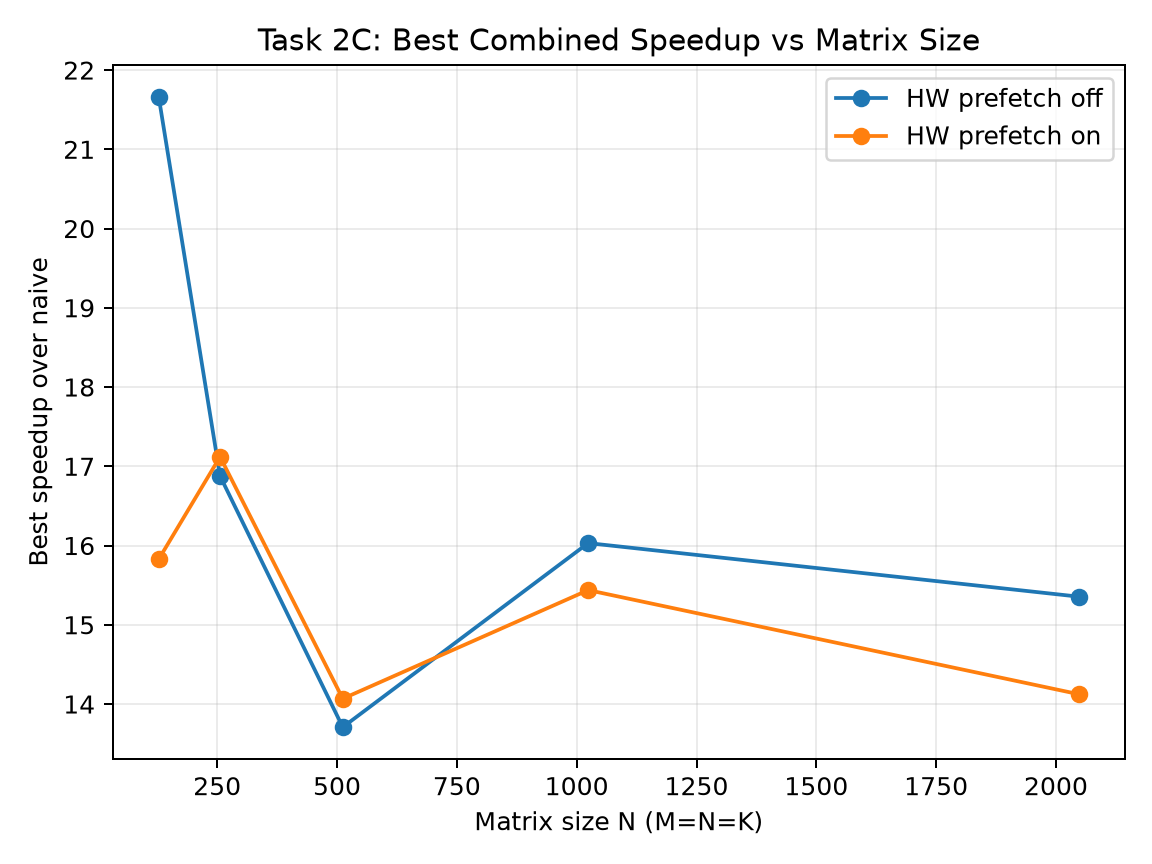
\includegraphics[width=\linewidth]{plots/task2c/task2c_best_speedup_vs_size.png}
        \caption{Combined Speedup vs. Matrix Size}
    \end{subfigure}
    \hfill
    \begin{subfigure}{0.48\textwidth}
        \centering
        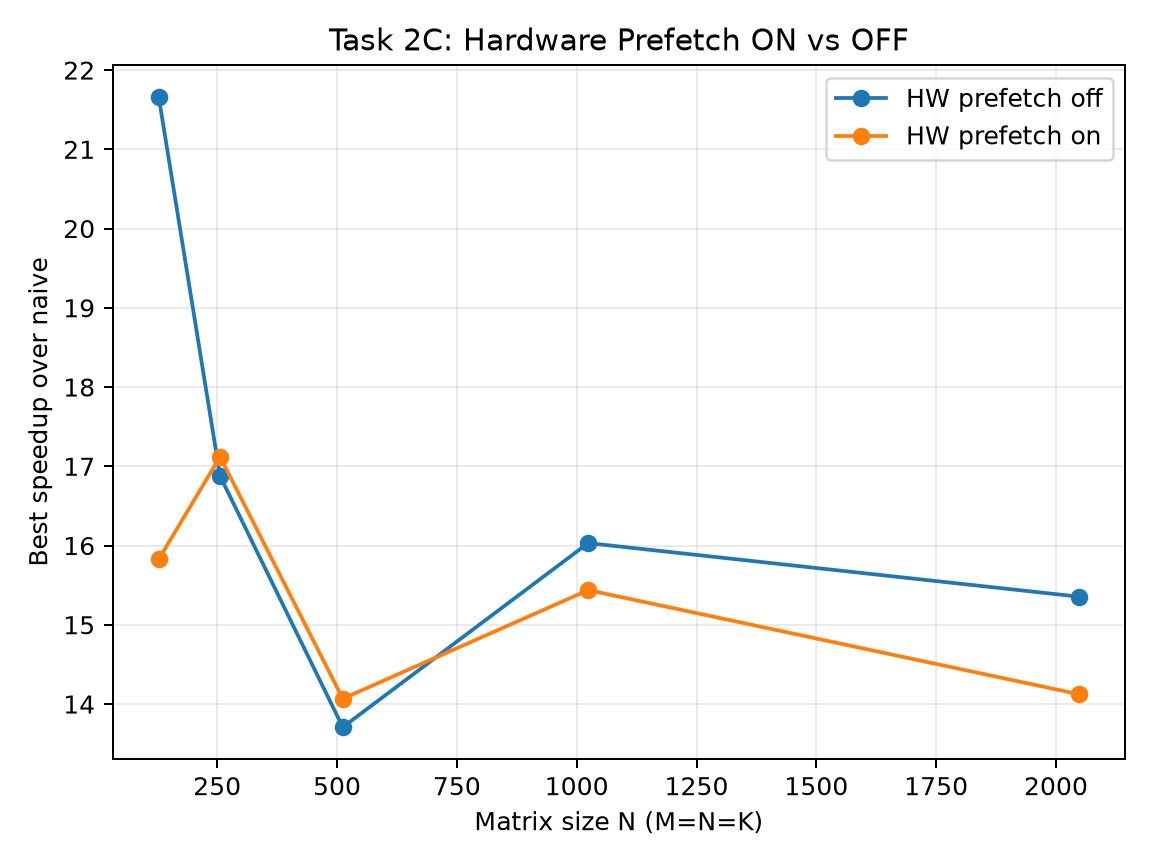
\includegraphics[width=\linewidth]{plots/task2c/task2c_hw_prefetch_on_off.png}
        \caption{Hardware Prefetcher ON vs OFF}
    \end{subfigure}
    \caption{Overall performance scaling of the combined optimizations.}
\end{figure}

\subsection{Analysis}

\subsubsection{SIMD Width and Instruction Count}
Moving from scalar code to 128-bit and then 256-bit SIMD drastically reduces the total number of instructions executed. Because the 256-bit SIMD instructions consume data much faster than scalar code (processing 8 floats per instruction), the CPU pipeline bottleneck shifts away from instruction fetch/decode and lands squarely on memory bandwidth.

\begin{figure}[H]
    \centering
    \begin{subfigure}{0.48\textwidth}
        \centering
        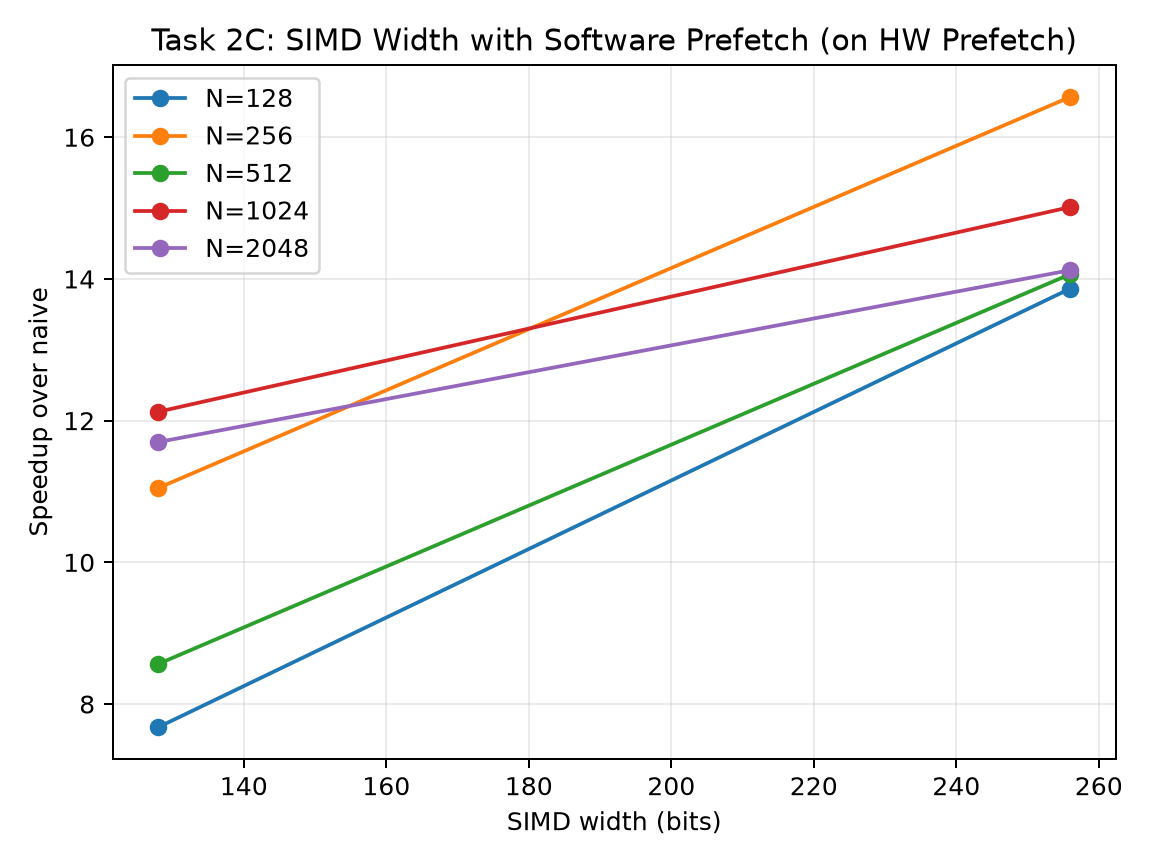
\includegraphics[width=\linewidth]{plots/task2c/task2c_simd_width.png}
        \caption{Speedup vs SIMD Width}
    \end{subfigure}
    \hfill
    \begin{subfigure}{0.48\textwidth}
        \centering
        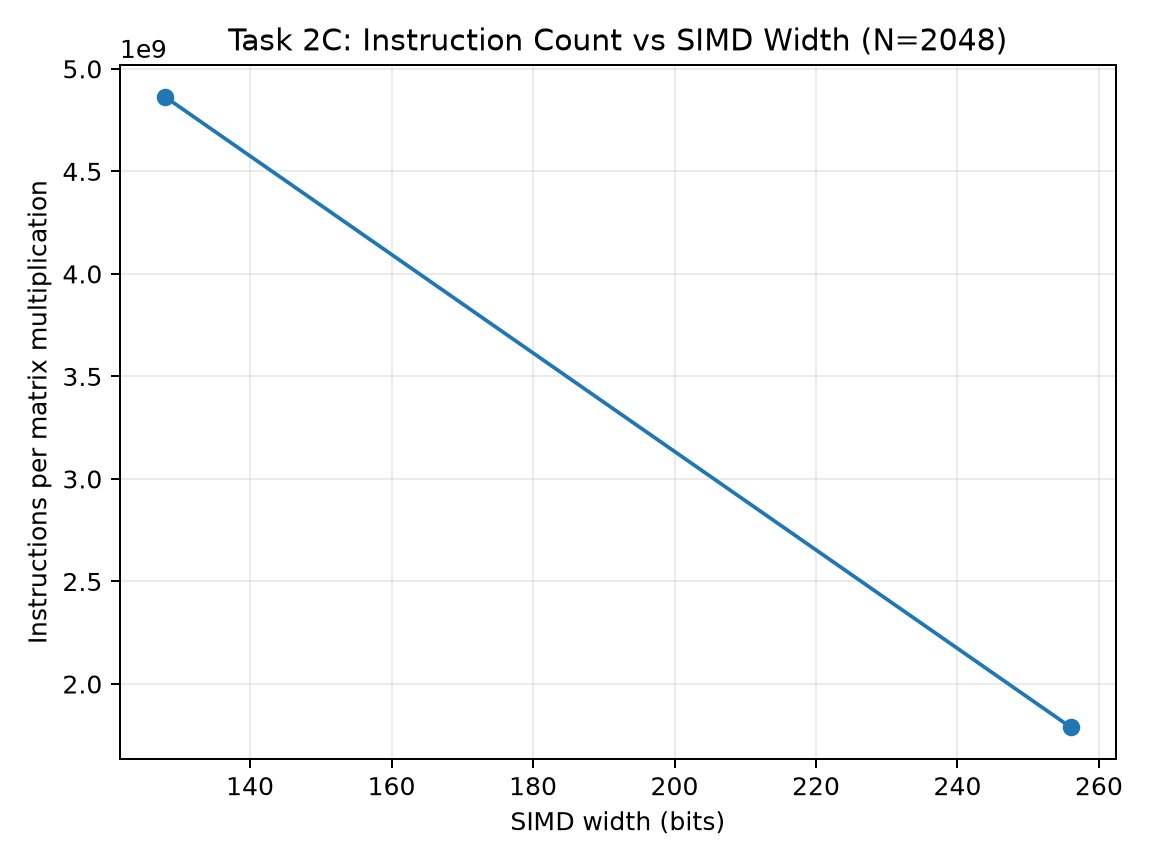
\includegraphics[width=\linewidth]{plots/task2c/task2c_instructions_vs_width.png}
        \caption{Instruction Count vs SIMD Width}
    \end{subfigure}
    \caption{Impact of expanding SIMD width on execution speed and instruction count.}
\end{figure}

\subsubsection{Prefetch Cache Fill Level}
Because of the massive throughput of the 256-bit ALUs, the kernel becomes highly sensitive to memory latency. Consequently, the optimal prefetch cache fill level shifted to \texttt{T0} (L1 cache) across almost all sizes. In Task 2A (scalar), \texttt{T1} (L2 cache) was preferred to avoid L1 thrashing. However, SIMD units require data immediately in the L1 cache; fetching to L2 introduces too much latency for the vector ALUs.

\begin{figure}[H]
\centering
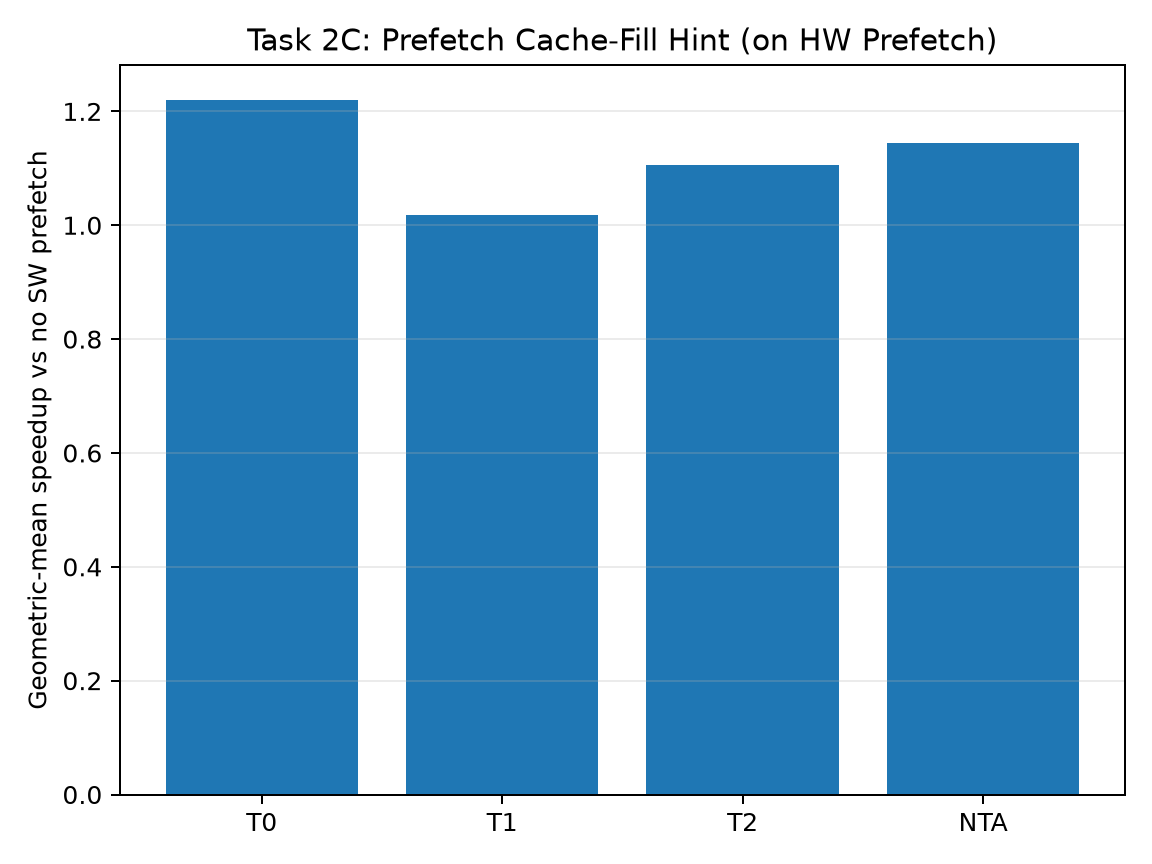
\includegraphics[width=0.6\linewidth]{plots/task2c/task2c_prefetch_level.png}
\caption{Speedup vs Cache Fill Hint (Geometric mean). \texttt{T0} provides the best performance for SIMD workloads.}
\end{figure}

\subsubsection{Prefetch Distance and Cache Metrics}
The geometric mean for the optimal prefetch distance landed at 32 floats, which ensures data arrives just in time without evicting the currently active $32 \times 32$ cache tiles. Requesting data too far ahead (e.g., 512 floats) triggers a noticeable increase in L1D and L2 cache misses, as prefetched data evicts active working sets before they can be fully utilized.

\begin{figure}[H]
\centering
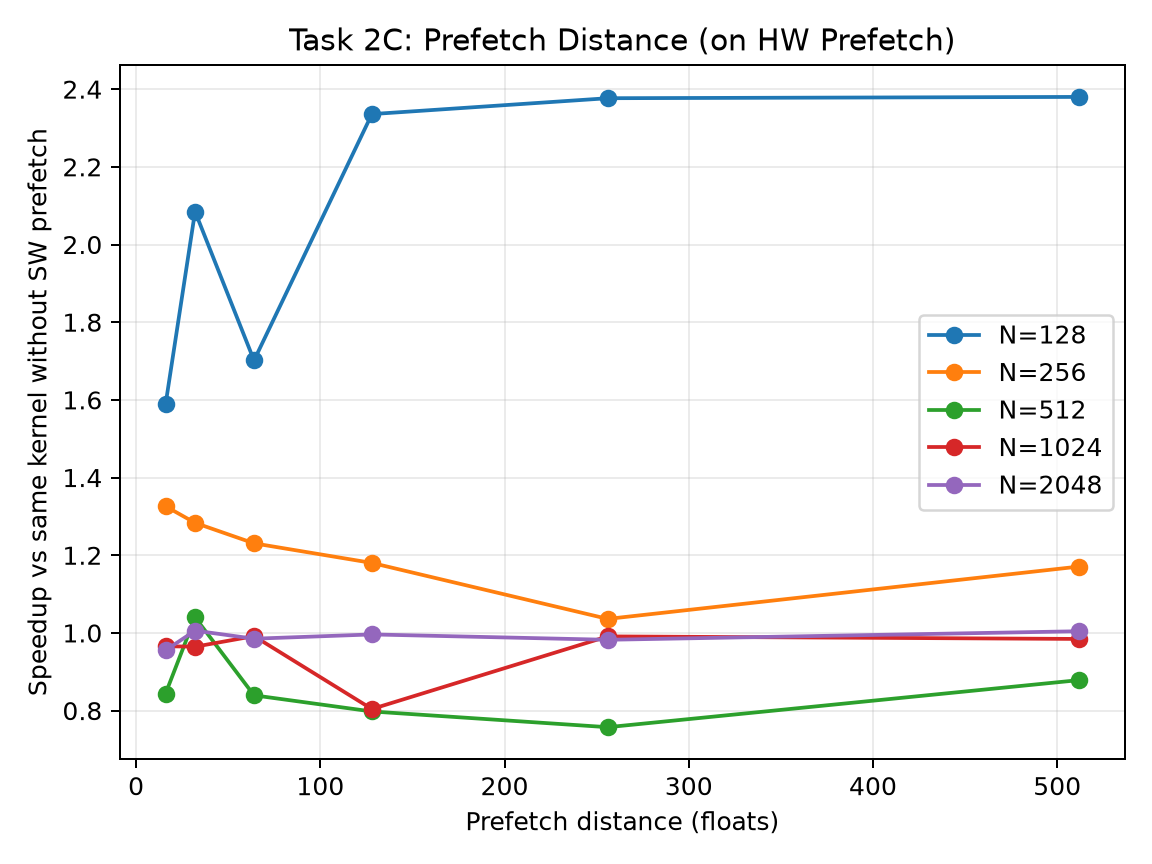
\includegraphics[width=0.65\linewidth]{plots/task2c/task2c_prefetch_distance.png}
\caption{Speedup over baseline (without SW prefetch) across varying prefetch distances.}
\end{figure}

\begin{figure}[H]
    \centering
    \begin{subfigure}{0.48\textwidth}
        \centering
        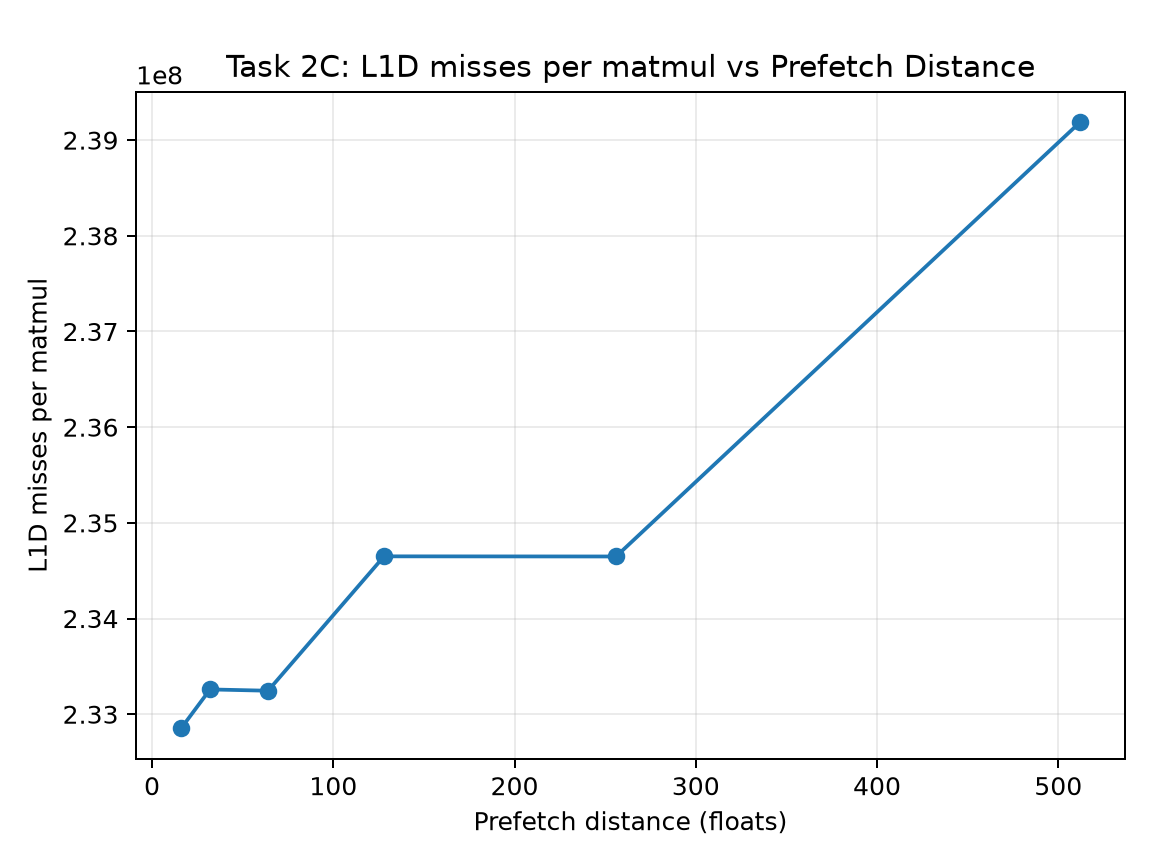
\includegraphics[width=\linewidth]{plots/task2c/task2c_l1d_misses_vs_distance.png}
        \caption{L1D Misses vs Distance}
    \end{subfigure}
    \hfill
    \begin{subfigure}{0.48\textwidth}
        \centering
        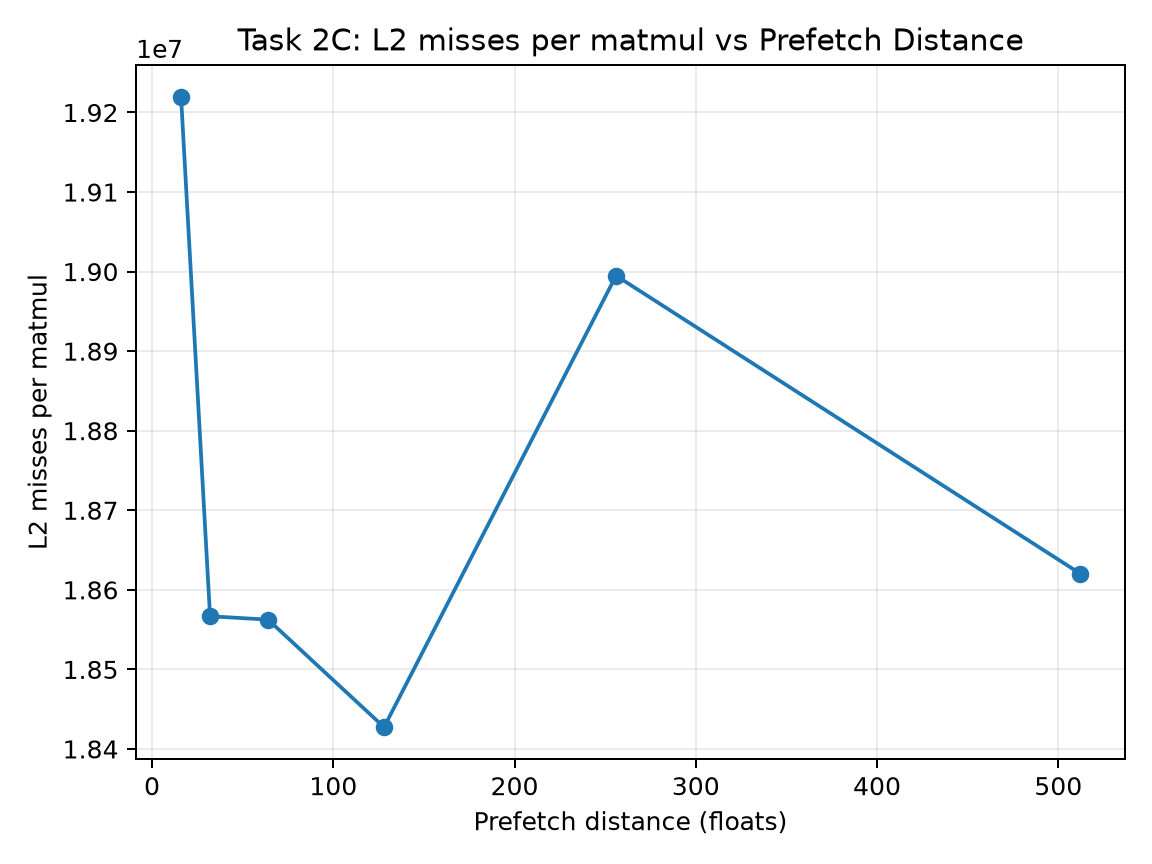
\includegraphics[width=\linewidth]{plots/task2c/task2c_l2_misses_vs_distance.png}
        \caption{L2 Misses vs Distance}
    \end{subfigure}
    \vspace{1em}
    \begin{subfigure}{0.48\textwidth}
        \centering
        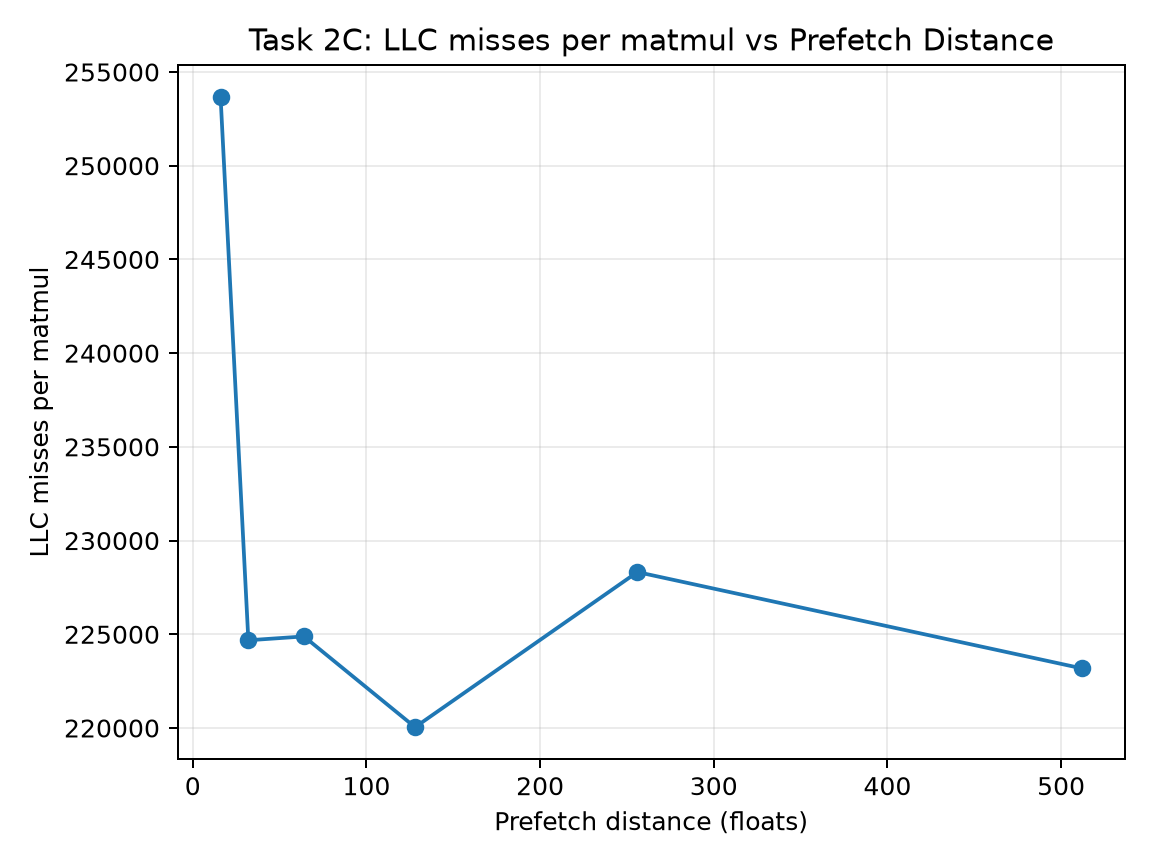
\includegraphics[width=\linewidth]{plots/task2c/task2c_llc_misses_vs_distance.png}
        \caption{LLC Misses vs Distance}
    \end{subfigure}
    \hfill
    \begin{subfigure}{0.48\textwidth}
        \centering
        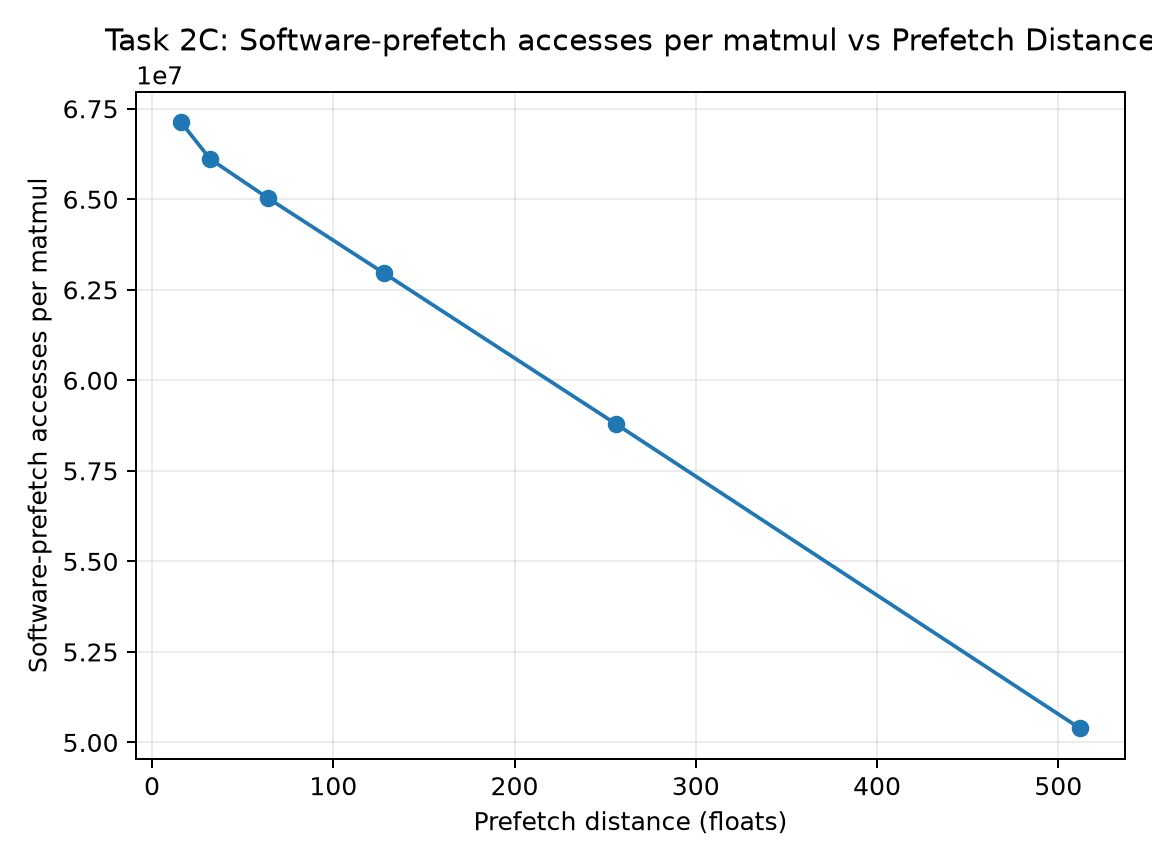
\includegraphics[width=\linewidth]{plots/task2c/task2c_sw_prefetch_access_vs_distance.png}
        \caption{SW Prefetch Accesses vs Distance}
    \end{subfigure}
    \caption{Hardware cache metrics behavior under varying prefetch distances ($N=2048$). Notice the spike in misses at extreme distances.}
\end{figure}

\subsection{Final Performance Comparison}

\begin{figure}[H]
\centering
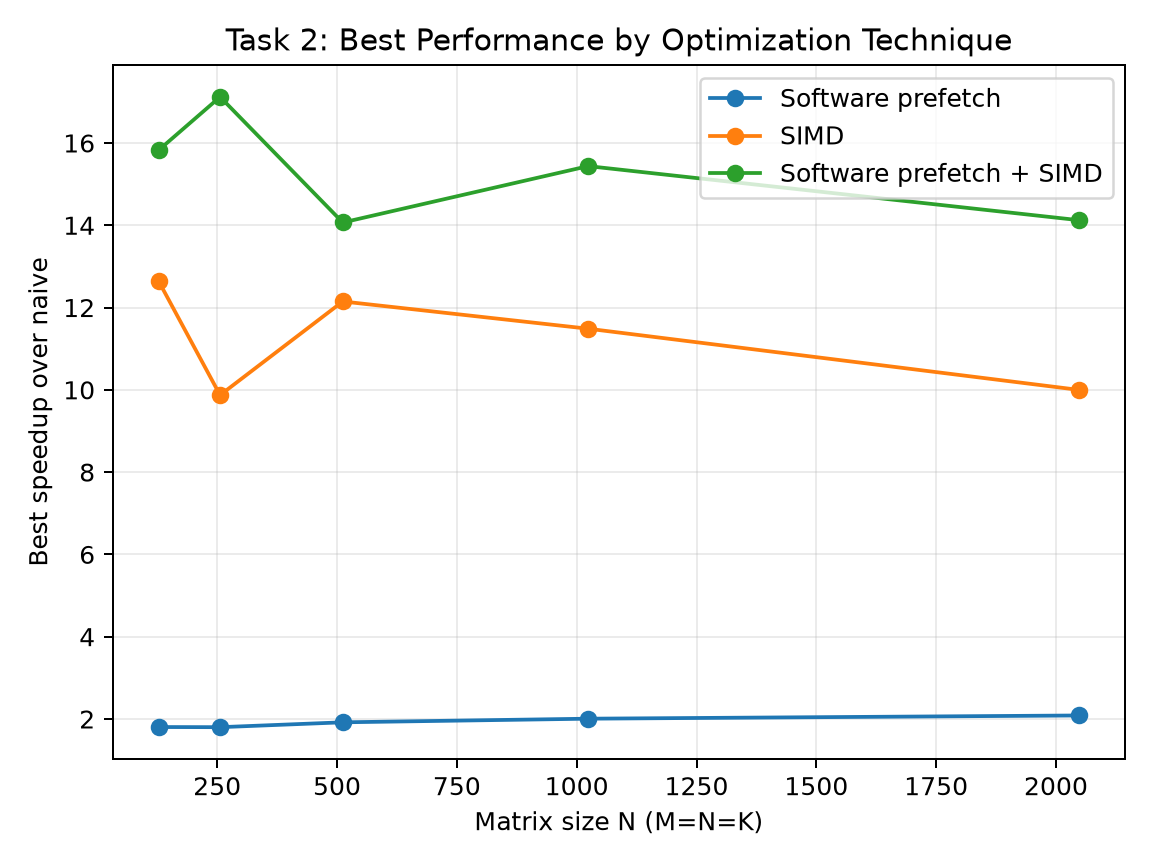
\includegraphics[width=0.8\linewidth]{plots/task2c/task2_final_best_comparison.png}
\caption{Task 2 final performance comparison across optimization techniques.}
\end{figure}

\begin{table}[H]
\centering
\caption{Task 2 final performance summary (Peak observed across sizes)}
\begin{tabular}{lllc}
\toprule
Technique & Peak Speedup & Optimal Hint/Width & Matrix Size at Peak \\
\midrule
Software Prefetching & $\sim 2.08\times$ & Distance 64, Hint T1 & $2048 \times 2048$ \\
SIMD                 & $\sim 12.6\times$ & 256-bit AVX2         & $128 \times 128$ \\
Prefetching + SIMD   & $17.11\times$     & 256-bit, Dist 16, T0 & $256 \times 256$ \\
\bottomrule
\end{tabular}
\end{table}

\subsection{Task 2 Conclusion}
The optimization journey clearly demonstrates that maximum performance requires harmonizing compute and memory architectures. While software prefetching alone provided a modest $\sim 2\times$ speedup by hiding latency, SIMD vectorization delivered a massive $>12\times$ compute boost. 

However, SIMD alone eventually stalls waiting for memory. By combining them—using cache tiling to shrink the working set, SIMD to maximize arithmetic throughput, and \texttt{T0} L1 software prefetching to guarantee data availability—we achieved a highly synergistic peak speedup of $17.11\times$. The combination proves that keeping vector units fed is just as critical as the vectorization itself.